\documentclass[tikz,border=10pt]{standalone}
% Shared look for every TikZ diagram. Load with % Shared look for every TikZ diagram. Load with % Shared look for every TikZ diagram. Load with \input{../../tools/tikz-style.tex}
\usepackage[T1]{fontenc}
\usepackage{lmodern}
\renewcommand{\sfdefault}{lmr}  % diagrams use the same serif as the text
\usetikzlibrary{arrows.meta, positioning, shapes.geometric, calc, fit, backgrounds}
\definecolor{cblue}{HTML}{4C78A8}
\definecolor{corange}{HTML}{F58518}
\definecolor{cgreen}{HTML}{54A24B}
\definecolor{cred}{HTML}{E45756}
\definecolor{cpurple}{HTML}{B279A2}
\definecolor{cgrey}{HTML}{6B6B6B}
\tikzset{
  every picture/.style={font=\sffamily, line width=1.2pt},
  box/.style={draw=#1, fill=#1!12, rounded corners=4pt, align=center, inner sep=7pt, minimum height=1.1cm},
  box/.default=cgrey,
  arrow/.style={-{Stealth[length=3mm]}, draw=cgrey, line width=1.4pt},
  title/.style={font=\sffamily\bfseries\Large},
  note/.style={font=\sffamily\small, text=cgrey, align=center},
}
\AtBeginDocument{\hyphenpenalty=10000 \exhyphenpenalty=10000}

\usepackage[T1]{fontenc}
\usepackage{lmodern}
\renewcommand{\sfdefault}{lmr}  % diagrams use the same serif as the text
\usetikzlibrary{arrows.meta, positioning, shapes.geometric, calc, fit, backgrounds}
\definecolor{cblue}{HTML}{4C78A8}
\definecolor{corange}{HTML}{F58518}
\definecolor{cgreen}{HTML}{54A24B}
\definecolor{cred}{HTML}{E45756}
\definecolor{cpurple}{HTML}{B279A2}
\definecolor{cgrey}{HTML}{6B6B6B}
\tikzset{
  every picture/.style={font=\sffamily, line width=1.2pt},
  box/.style={draw=#1, fill=#1!12, rounded corners=4pt, align=center, inner sep=7pt, minimum height=1.1cm},
  box/.default=cgrey,
  arrow/.style={-{Stealth[length=3mm]}, draw=cgrey, line width=1.4pt},
  title/.style={font=\sffamily\bfseries\Large},
  note/.style={font=\sffamily\small, text=cgrey, align=center},
}
\AtBeginDocument{\hyphenpenalty=10000 \exhyphenpenalty=10000}

\usepackage[T1]{fontenc}
\usepackage{lmodern}
\renewcommand{\sfdefault}{lmr}  % diagrams use the same serif as the text
\usetikzlibrary{arrows.meta, positioning, shapes.geometric, calc, fit, backgrounds}
\definecolor{cblue}{HTML}{4C78A8}
\definecolor{corange}{HTML}{F58518}
\definecolor{cgreen}{HTML}{54A24B}
\definecolor{cred}{HTML}{E45756}
\definecolor{cpurple}{HTML}{B279A2}
\definecolor{cgrey}{HTML}{6B6B6B}
\tikzset{
  every picture/.style={font=\sffamily, line width=1.2pt},
  box/.style={draw=#1, fill=#1!12, rounded corners=4pt, align=center, inner sep=7pt, minimum height=1.1cm},
  box/.default=cgrey,
  arrow/.style={-{Stealth[length=3mm]}, draw=cgrey, line width=1.4pt},
  title/.style={font=\sffamily\bfseries\Large},
  note/.style={font=\sffamily\small, text=cgrey, align=center},
}
\AtBeginDocument{\hyphenpenalty=10000 \exhyphenpenalty=10000}

\begin{document}
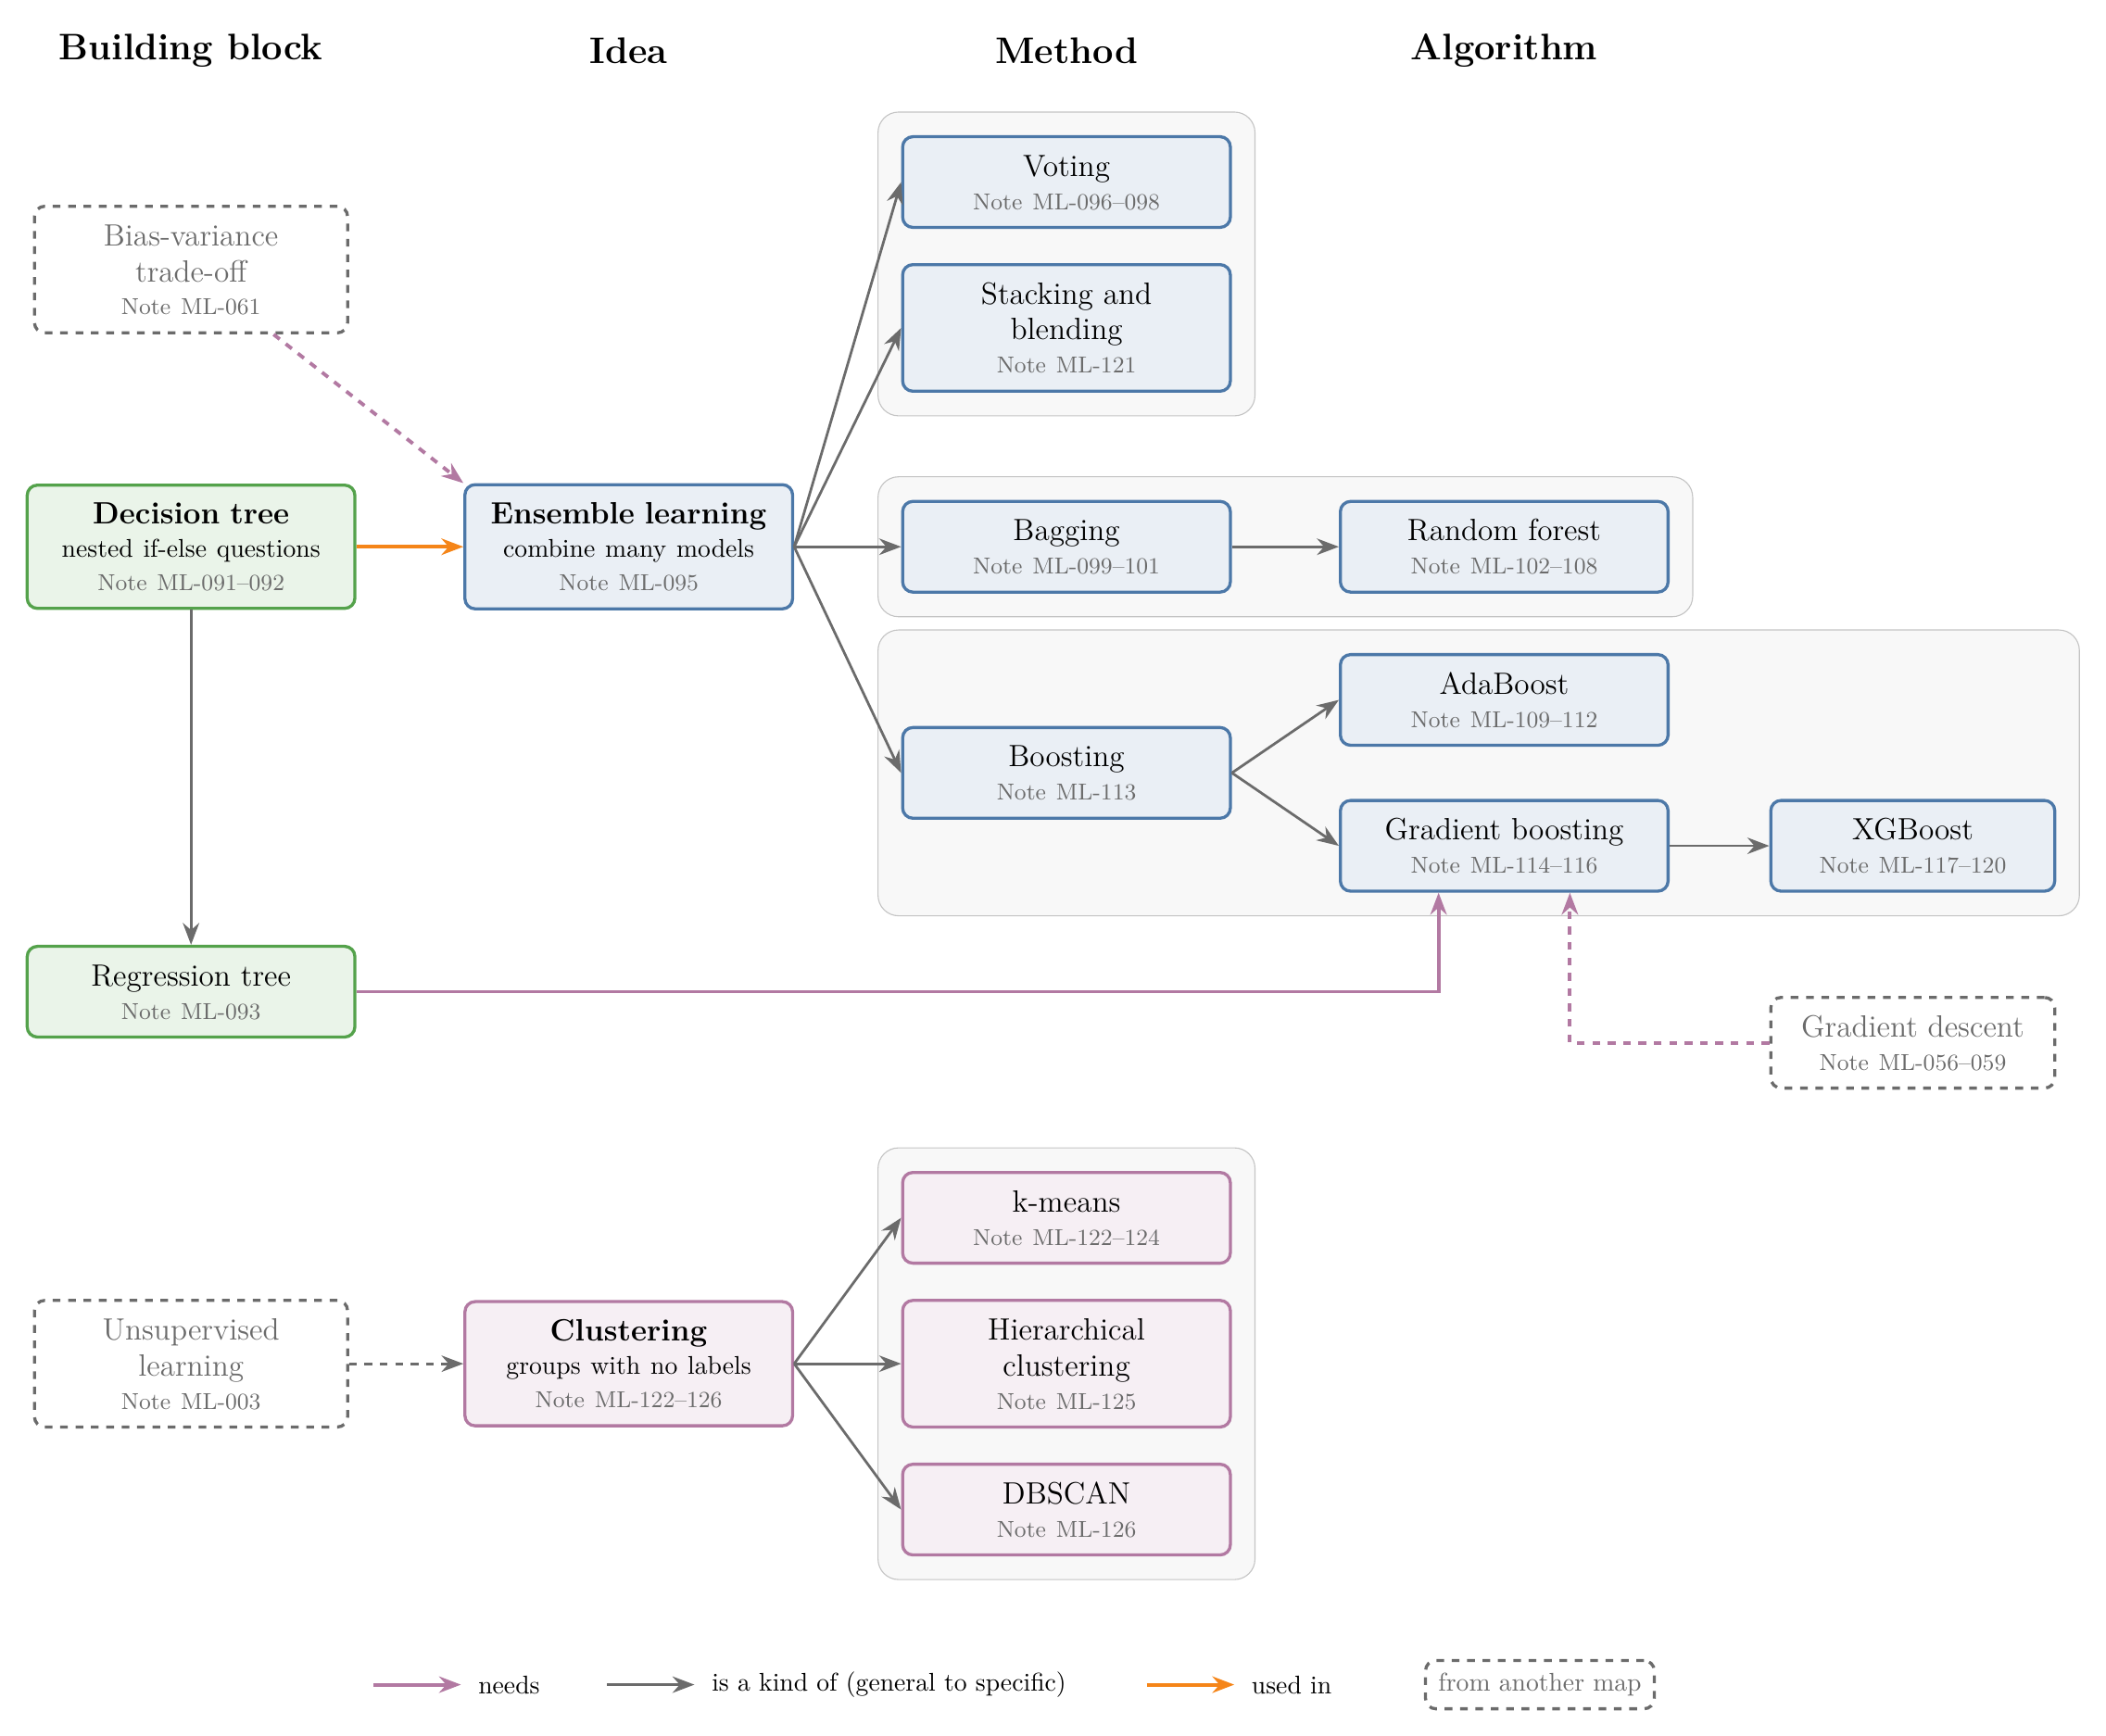
\begin{tikzpicture}[
    every node/.append style={font=\sffamily\large},
    con/.style={box=cblue, text width=4.0cm},
    prob/.style={box=cred, text width=4.0cm},
    prev/.style={draw=cgrey, dashed, rounded corners=4pt, align=center, inner sep=7pt, text=cgrey, text width=3.8cm, minimum height=1.1cm},
    group/.style={draw=cgrey!40, fill=cgrey!5, rounded corners=8pt, inner sep=9pt},
    kind/.style={arrow, draw=cgrey, line width=1pt},
    needs/.style={arrow, draw=cpurple},
    fixes/.style={arrow, draw=cgreen},
    usedin/.style={arrow, draw=corange},
  ]
  \newcommand{\nt}[1]{\\[-1pt]{\small\color{cgrey}Note #1}}
  \newcommand{\sub}[1]{\\[-1pt]{\normalsize #1}}
  \node[title] at (0,11.4) {Building block};
  \node[title] at (6,11.4) {Idea};
  \node[title] at (12,11.4) {Method};
  \node[title] at (18,11.4) {Algorithm};

  % building blocks
  \node[box=cgreen, text width=4.0cm] (dt) at (0,4.6) {\textbf{Decision tree}\sub{nested if-else questions}\nt{ML-091--092}};
  \node[box=cgreen, text width=4.0cm] (rt) at (0,-1.5) {Regression tree\nt{ML-093}};
  \node[prev] (bv) at (0,8.4) {Bias-variance trade-off\nt{ML-061}};
  \draw[kind] (dt) -- (rt);

  % ensembles
  \node[con] (ens) at (6,4.6) {\textbf{Ensemble learning}\sub{combine many models}\nt{ML-095}};
  \node[con] (vote) at (12,9.6) {Voting\nt{ML-096--098}};
  \node[con] (stack) at (12,7.6) {Stacking and blending\nt{ML-121}};
  \node[con] (bag) at (12,4.6) {Bagging\nt{ML-099--101}};
  \node[con] (boost) at (12,1.5) {Boosting\nt{ML-113}};
  \node[con] (rf) at (18,4.6) {Random forest\nt{ML-102--108}};
  \node[con] (ada) at (18,2.5) {AdaBoost\nt{ML-109--112}};
  \node[con] (gb) at (18,0.5) {Gradient boosting\nt{ML-114--116}};
  \node[con, text width=3.4cm] (xgb) at (23.6,0.5) {XGBoost\nt{ML-117--120}};
  \node[prev, text width=3.4cm] (gd) at (23.6,-2.2) {Gradient descent\nt{ML-056--059}};

  \begin{scope}[on background layer]
    \node[group, fit=(vote) (stack)] {};
    \node[group, fit=(bag) (rf)] {};
    \node[group, fit=(boost) (ada) (gb) (xgb)] {};
  \end{scope}

  \draw[usedin] (dt) -- (ens);
  \draw[needs, dashed] (bv) -- (ens.north west);
  \foreach \m in {vote, stack, bag, boost} \draw[kind] (ens.east) -- (\m.west);
  \draw[kind] (bag) -- (rf);
  \draw[kind] (boost.east) -- (ada.west);
  \draw[kind] (boost.east) -- (gb.west);
  \draw[kind] (gb) -- (xgb);
  \draw[needs] (rt.east) -| ([xshift=-0.9cm]gb.south);
  \draw[needs, dashed] (gd.west) -| ([xshift=0.9cm]gb.south);

  % clustering
  \node[prev] (unsup) at (0,-6.6) {Unsupervised learning\nt{ML-003}};
  \node[box=cpurple, text width=4.0cm] (clu) at (6,-6.6) {\textbf{Clustering}\sub{groups with no labels}\nt{ML-122--126}};
  \node[box=cpurple, text width=4.0cm] (km) at (12,-4.6) {k-means\nt{ML-122--124}};
  \node[box=cpurple, text width=4.0cm] (hc) at (12,-6.6) {Hierarchical clustering\nt{ML-125}};
  \node[box=cpurple, text width=4.0cm] (db) at (12,-8.6) {DBSCAN\nt{ML-126}};
  \begin{scope}[on background layer]
    \node[group, fit=(km) (hc) (db)] {};
  \end{scope}
  \draw[kind, dashed] (unsup) -- (clu);
  \foreach \m in {km, hc, db} \draw[kind] (clu.east) -- (\m.west);

  % legend
  \begin{scope}[shift={(2.5,-11.0)}, every node/.style={font=\sffamily, anchor=west}]
    \draw[needs] (0,0) -- (1.2,0);      \node at (1.3,0) {needs};
    \draw[kind] (3.2,0) -- (4.4,0);     \node at (4.5,0) {is a kind of (general to specific)};
    \draw[usedin] (10.6,0) -- (11.8,0); \node at (11.9,0) {used in};
    \node[draw=cgrey, dashed, rounded corners=4pt, inner sep=5pt, text=cgrey, anchor=west] at (14.4,0) {from another map};
  \end{scope}
\end{tikzpicture}
\end{document}
